
%\RequirePackage{pdf15}

\documentclass{beamer}

\usepackage[utf8]{inputenc}

\usepackage{mystyle}

\usepackage{natbib}
\usepackage{tikz}
\usepackage{pgfplots}
\usepackage{subcaption}

\usepackage{tikz-dependency}
\usetikzlibrary{shapes.arrows, positioning, fit, bayesnet,
    arrows,backgrounds,patterns,matrix,calc,shadows,plotmarks,
    shapes,positioning,automata,positioning,spy,scopes,chains,decorations,decorations.pathreplacing}

\newcommand{\FancyUpArrow}{
\begin{tikzpicture}[baseline=-0.3em]
\node[single arrow,draw,rotate=90,single arrow head extend=0.2em,inner
ysep=0.2em,transform shape,line width=0.05em,top color=green,bottom color=green!50!black] (X){};
\end{tikzpicture}}
\newcommand{\FancyDownArrow}{
\begin{tikzpicture}[baseline=-0.3em]
\node[single arrow,draw,rotate=-90,single arrow head extend=0.2em,inner
ysep=0.2em,transform shape,line width=0.05em,top color=red,bottom color=red!50!black] (X){};
\end{tikzpicture}}

%Information to be included in the title page:
\title{Scaling Hidden Markov Language Models}
\author{Anonymous}
\date{2020}



\begin{document}

\frame{\titlepage}

\begin{frame}
\frametitle{Hidden Markov Models in NLP}
\begin{itemize}
\item Historically significant latent variable models
    \begin{itemize}
    \item Applied to tagging, alignment, and language modeling in the 90s
    \end{itemize}
\item Are thought to be very poor language models
    \begin{itemize}
    \item We show they are not!
    \end{itemize}
\end{itemize}
\end{frame}

\begin{frame}
\frametitle{Lessons from Large Neural Language Models}

Large models perform better but are \ldots

\begin{itemize}
\item Slow to train
    \begin{itemize}
    \item Parallelize computation and use GPUs
    \end{itemize}
\item Prone to overfitting
    \begin{itemize}
    \item Regularize
    \end{itemize}
\end{itemize}

Apply this to scaling HMMs
% Before we get into how we apply these lessons to HMMs,
% lets briefly review HMMs to see why they present different challenges than
% other neural language models
\end{frame}

\begin{frame}
\frametitle{HMMs}

For times $t \in [T]$, model states $z_t \in \mcZ$ and tokens $x_t \in \mcX$

\begin{center}
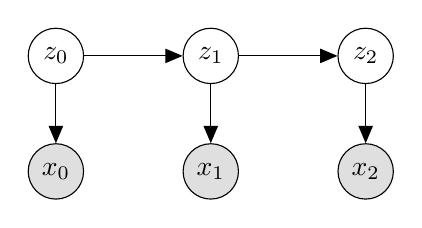
\begin{tikzpicture}[]
\node[latent] (z0) {$z_0$} ;
\node[latent] (z1) [right=1.25cm of z0] {$z_1$} ;
\node[latent] (z2) [right=1.25cm of z1] {$z_2$} ;

\node[obs]    (x0) [below = 0.75cm of z0] {$x_0$};
\node[obs]    (x1) [below = 0.75cm of z1] {$x_1$};
\node[obs]    (x2) [below = 0.75cm of z2] {$x_2$};

\edge {z0} {x0};
\edge {z1} {x1};
\edge {z2} {x2};
\edge {z0} {z1};
\edge {z1} {z2};
\end{tikzpicture}
\end{center}

%\begin{equation*}
%p(\bx,\bz) = \prod_{t=1}^T 
    %\underbrace{p(z_t \mid z_{t-1})}_{\textrm{transition}}
    %\underbrace{p(x_t\mid z_t)}_{\textrm{emission}}
%\end{equation*}

We wish optimize
\begin{equation*}
p(\bx) = \sum_\bz p(\bx,\bz)
\end{equation*}
\end{frame}

\begin{frame}
\frametitle{3 Tricks for Training Large HMMs}
\begin{itemize}
\item Block-sparse emission constraints
    \begin{itemize}
    \item[] \FancyUpArrow~Speed
    \end{itemize}
\item Compact neural parameterization
    \begin{itemize}
    \item[] \FancyUpArrow~Generalization
    \end{itemize}
\item State dropout
    \begin{itemize}
    \item[] \FancyUpArrow~Speed \FancyUpArrow~Generalization
    \end{itemize}
\end{itemize}
\end{frame}

\begin{frame}
\frametitle{Block-Sparse Emission Constraints}
\begin{itemize}
\item Partition words and states jointly
\item Words can only be emit by states in same group
\end{itemize}
\begin{center}
\begin{tikzpicture}[every node/.style={anchor=base,minimum size=8mm}]
    \matrix  (graph) [matrix of nodes, row sep=0.5em,column sep=-0.3em,
    minimum width=2em, minimum height=2em, font=\small,ampersand replacement=\&,
    nodes in empty cells
    ] {
        \&$\mcX_1$ \&
        \&
        \textcolor{green!10}{a}\&
        $\mcX_2$ \&
        \textcolor{green!10}{a}\&
        \&
        $\cdots$ \&
        \&
        $\mcX_M$ \\
        \textcolor{blue!80}{$p(x\mid z)$} \& \& \& \&\& \&\&\&\&\\
        \&$\mcZ_1$ \&
        \&
        $\mcZ_2$ \&
        \&
        $\cdots$ \&
        \&
        $\mcZ_M$ \&\&\\
    };
    
    \begin{scope}[on background layer]
      \draw[blue!30, line width=0.5mm] (graph-1-2) -- (graph-3-2);
      \draw[blue!30,line width=0.5mm] (graph-1-5) -- (graph-3-4);
      \draw[blue!30,line width=0.5mm] (graph-1-10) -- (graph-3-8);

      %\draw[draw=red!30, line width=0.2mm] ($(graph-1-1) + (0.1, 0)$) -- ($(graph-3-3) + (0.1, 0)$);
      %\draw[draw=red!30, line width=0.2mm] ($(graph-1-2) + (0.1, 0)$) -- ($(graph-3-3) + (0.1, 0)$);
      %\draw[draw=red!30, line width=0.1mm] ($(graph-1-3) + (0.1, 0)$) -- ($(graph-3-3) + (0.1, 0)$);
      %\draw[draw=red!30, line width=0.9mm] ($(graph-1-4) + (0.1, 0)$) -- ($(graph-3-3) + (0.1, 0)$);
      %\draw[draw=red!30, line width=0.1mm] ($(graph-1-5) + (0.1, 0)$) -- ($(graph-3-3) + (0.1, 0)$);
      %\draw[draw=red!30, line width=0.4mm] ($(graph-1-6) + (0.1, 0)$) -- ($(graph-3-3) + (0.1, 0)$);
      %\draw[draw=red!30, line width=0.1mm] ($(graph-1-7) + (0.1, 0)$) -- ($(graph-3-3) + (0.1, 0)$);

      \draw[rounded corners,fill=red!10] ($ (graph-3-2.north west) +(-0.1,0.1)$) rectangle  node[yshift=-0.8cm]{\textcolor{red}{}} ($(graph-3-8.south east) +(0.1,-0.1)$ ) ;
      \draw[rounded corners,fill=red!10] ($ (graph-1-2.north west) +(-0.1,0.1)$) rectangle  node[yshift=0.8cm]{\textcolor{red}{}} ($(graph-1-10.south east) +(0.1,-0.1)$ ) ;

      \draw[rounded corners,fill=green!10] (graph-1-2.north west) rectangle  node[ yshift =0.7cm] {} (graph-1-2.south east);
      \draw[rounded corners,fill=green!10] (graph-1-4.north west) rectangle  node[ yshift =0.7cm] {} (graph-1-6.south east);
      \draw[rounded corners,fill=green!10] (graph-1-10.north west) rectangle  node[ yshift =0.7cm] {} (graph-1-10.south east);

      \draw[rounded corners, fill=blue!10] (graph-3-2.north west) rectangle  node[yshift=-0.9cm]{}  ($(graph-3-2.south east)$);
      \draw[rounded corners, fill=blue!10] (graph-3-4.north west) rectangle  node[yshift=-0.9cm]{}  ($(graph-3-4.south east)$);
      \draw[rounded corners,fill=blue!10] (graph-3-8.north west) rectangle  node[ yshift =0.7cm] {} (graph-3-8.south east);
      %\path[] (graph-3-3.north west) rectangle  node[yshift=-0.9cm]{\textbf{$y_3$}} (graph-3-3.south east);
    \end{scope}
  \end{tikzpicture}
\end{center}

\end{frame}

\begin{frame}
\frametitle{Block-Sparse Emissions: Effect on Inference}

\begin{figure}
\captionsetup[subfigure]{justification=centering}
\begin{center}
\begin{subfigure}[t]{0.45\textwidth}
\centering
\resizebox{0.75\width}{0.75\height}{
\input{img/diagram_full.tex}
}
\caption{No constraints}
\end{subfigure}
\begin{subfigure}[t]{0.45\textwidth}
\centering
\resizebox{0.75\width}{0.75\height}{
\input{img/trellis_nodrop.tex}
}
\caption{Block-sparse emission constraints}
\end{subfigure}
\end{center}
\end{figure}

After observing each $x_t$, only the states in the corresponding group have nonzero probability
of occurring
\end{frame}

\begin{frame}
\frametitle{Neural Parameterization}
Generate transition and emission distributions using a neural network
\begin{itemize}
\item State embeddings $\mathbf{E}_z \in \mathbb{R}^{|\mcZ| \times h}$
\item Token embeddings $\mathbf{E}_x \in \mathbb{R}^{|\mcX| \times h}$
\end{itemize}
\vspace{0.5em}
\centering
\includegraphics[height=1.7in]{img/blocksparse_mat_no_block.pdf}
\end{frame}

\begin{frame}
\frametitle{State Dropout}
At each batch, sample dropout mask $\mathbf{b} \in \set{0,1}^{|\mcZ|}$
\vspace{1em}
\begin{center}
\resizebox{0.75\width}{0.75\height}{
\input{img/trellis.tex}
}
\end{center}
\end{frame}

\begin{frame}
\frametitle{Experiments}
\begin{itemize}
\item Language modeling on Penn Treebank and Wikitext-2
\item Baselines
    \begin{itemize}
    \item Knesey-Ney 5-gram model
    \item Feedforward 5-gram model
    \item 2-layer LSTM
    \end{itemize}
\item Model
    \begin{itemize}
    \item $2^{15}$ (32k) state very large HMM (VL-HMM)
    \item $M=128$ groups (256 states each), obtained via Brown Clustering
    \item Dropout rate of $0.5$ during training
    \end{itemize}
\end{itemize}
\end{frame}

\begin{comment}
\begin{frame}
\frametitle{Results on PTB and WT2}
\centering
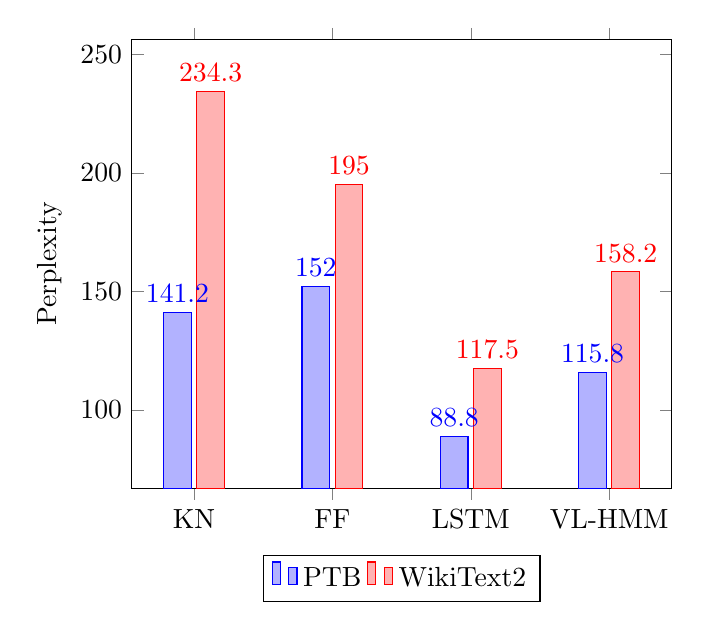
\begin{tikzpicture}
\begin{axis}[
    ybar,
    enlargelimits=0.15,
    legend style={at={(0.5,-0.15)},
      anchor=north,legend columns=-1},
    ylabel={Perplexity},
    symbolic x coords={KN, FF, LSTM, VL-HMM},
    xtick=data,
    nodes near coords,
    nodes near coords align={vertical},
    ]
\addplot coordinates {(KN,141.2) (FF,152.0) (LSTM,88.8) (VL-HMM,115.8)};
\addplot coordinates {(KN,234.3) (FF,195.0) (LSTM,117.5) (VL-HMM,158.2)};
\legend{PTB,WikiText2}
\end{axis}
\end{tikzpicture}
\end{frame}
\end{comment}

\begin{frame}
\frametitle{Results on PTB and WT2}
\centering
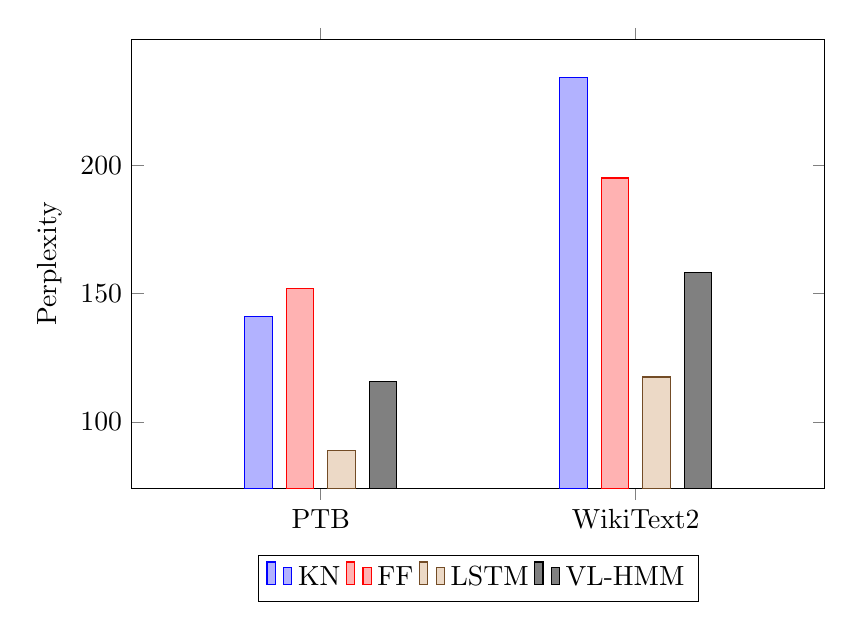
\begin{tikzpicture}
\begin{axis}[
    ybar=5pt,
    x=4cm,
    enlarge x limits=0.6,
    legend style={at={(0.5,-0.15)},
      anchor=north,legend columns=-1},
    ylabel={Perplexity},
    symbolic x coords={PTB, WikiText2},
    xtick=data,
    %nodes near coords,
    %nodes near coords align={vertical},
    bar width=10 pt,
    ]

\addplot coordinates {(PTB,141.2) (WikiText2,234.3)};
\addplot coordinates {(PTB,152.0) (WikiText2,195.0)};
\addplot coordinates {(PTB,88.8) (WikiText2,117.5)};
\addplot coordinates {(PTB,115.8) (WikiText2,158.2)};

\legend{KN, FF, LSTM, VL-HMM}
\end{axis}
\end{tikzpicture}
\end{frame}

\begin{comment}
\begin{frame}
\frametitle{Results on PTB}

\begin{table}[!t]
\centering
\begin{tabular}{llrr}
\toprule
Model & \# Params & Val PPL  & Test PPL\\
\midrule
KN 5-gram   & 2M & - & 141.2\\
256 FF 5-gram  & 2.9M     & 159.9      & 152.0  \\
AWD-LSTM  & 24M & 60.0 & 57.3\\
2x256 dim LSTM  & 3.6M     & 93.6       & 88.8   \\
%HMM+RNN   & 10M & 142.3 & -\\
HMM ($|\mcZ|$=900) & 10M & 284.6 & -\\
VL-HMM ($|\mcZ|=2^{15}$)   & 7.7M     & 125.0      & 115.8  \\
\bottomrule
\end{tabular}
\end{table}

\end{frame}

\begin{frame}
\frametitle{Results on WikiText2}

\begin{table}[!t]
\centering
\begin{tabular}{llrr}
\toprule
Model & \# Param & Val PPL & Test PPL\\
\midrule
KN 5-gram & 5.7M       & 248.7 & 234.3\\
AWD-LSTM & 33M & 68.6 & 65.8\\
256 FF 5-gram        & 8.8M    & 210.9  & 195.0\\
2x256  LSTM     & 9.6M    & 124.5  & 117.5\\
%32k state HMM (no fac)   & 17.3M   & 166.7  & -\\
VL-HMM ($|\mcZ|=2^{15}$)           & 13.7M   & 169.0      & 158.2\\
\bottomrule
\end{tabular}
\end{table}
\end{frame}
\end{comment}

\begin{frame}
\frametitle{State Size Ablation}

\centering
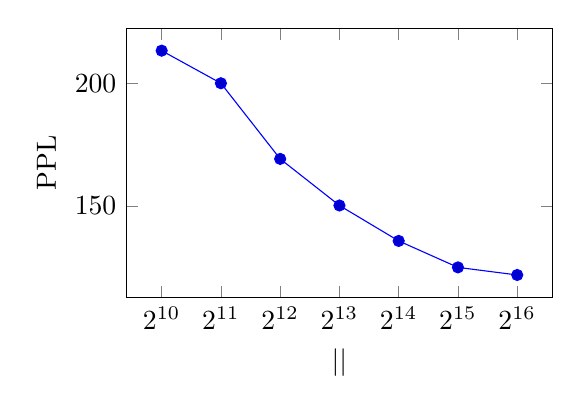
\begin{tikzpicture}
\begin{axis}[
    xlabel=$|\mcZ|$,
    ylabel=PPL,
    xmode=log,
    log basis x={2},
    xtick={},
    width=7cm,
    height=5cm
]
\addplot plot coordinates {
(1024,  213.25)
(2048,  199.98)
(4096,  169.18)
(8192,  150.22)
(16384, 135.79)
(32768, 125.02)
(65536, 121.93)
};
\end{axis}
\end{tikzpicture}

Perplexity on PTB by state size $|\mcZ|$ ($\lambda =0.5$ and $M=128$)
\end{frame}

\begin{frame}
\frametitle{Other Ablations}

\begin{center}
\begin{tabular}{lrrrr}
\toprule
Model                & Param & Train  & Val  &  Time \\
\midrule
VL-HMM ($2^{14}$)    & 7.2M & 115    & 134  & 40\\
\quad - neural param & 423M & 119    & 169  & 14\\
\quad - state dropout      & 7.2M & 88     & 157  & 100\\
\bottomrule
\end{tabular}
\end{center}
\end{frame}


\begin{frame}
\frametitle{Conclusion}
\begin{itemize}
\item HMMs can be scaled up to be competitive language models
\item Introduced 3 tricks for tackling speed and overfitting
\item HMMs are cool!
\end{itemize}
\end{frame}

\begin{frame}
\frametitle{EOS}
\end{frame}


\begin{frame}
\frametitle{Citations}
\bibliographystyle{acl_natbib}
\bibliography{anthology,emnlp2020}
\end{frame}

\end{document}
